\chapter{Diseño Metodológico}
\label{chap:metodologia}

Este capítulo detalla el diseño, implementación y evaluación del modelo de simulación. La metodología se divide en tres fases: modelado conceptual (sección \ref{sec:conceptual-modeling}), implementación del prototipo (sección \ref{sec:implementation}), y evaluación experimental (sección \ref{sec:validation-experimentation}).

\section{Fase 1: Modelo Conceptual}
\label{sec:conceptual-modeling}

\subsection{Límites del modelo (system boundary)}
\label{sec:limites-supuestos}

El modelo se centra en el nodo de almacenamiento primario de Coyhaique (431 TM: Abastible 150, Lipigas 240, Gasco 41). Un quiebre de stock en este nodo implica incapacidad de abastecer al resto de la región.

\textbf{Dentro del modelo:}
\begin{itemize}
    \item Dinámica de inventario del hub Coyhaique (agregado de 3 plantas)
    \item Flujo de suministro desde Cabo Negro/Neuquén (lead time: 6 días)
    \item Demanda agregada regional (52,5 TM/día)
    \item Disrupciones de la Ruta 7 (frecuencia y duración estocásticas)
\end{itemize}

\textbf{Fuera del modelo:}
\begin{itemize}
    \item Distribución de última milla a localidades remotas
    \item Inventarios individuales por distribuidor (modelo agrega los tres)
    \item Dinámicas competitivas entre Abastible, Lipigas y Gasco
\end{itemize}

\subsection{Diagrama conceptual del sistema}

La Figura~\ref{fig:conceptual-diagram-detailed} muestra la estructura completa del modelo conceptual del sistema de distribución de GLP en Aysén. El diagrama distingue cuatro tipos de elementos mediante colores: el flujo operacional (azul) que conecta suministro, almacenamiento y demanda; las disrupciones exógenas (rosa/terracota) que afectan el lead time; los parámetros configurables (gris) que definen la política de inventario; y la métrica de resiliencia (borgoña) que mide el desempeño del sistema. La política $(Q,R)$ controla el reabastecimiento basándose en el nivel de inventario, mientras que las disrupciones estocásticas introducen variabilidad en el lead time de transporte.

\begin{figure}[htbp]
    \centering
    \begin{tikzpicture}[
        font=\sffamily\small,
        scale=0.95,
        node distance=5cm,
        box/.style = {rectangle, draw=black!50, line width=1.5pt, rounded corners=3pt,
                     minimum height=2cm, minimum width=3cm,
                     text centered, font=\sffamily\small, align=center},
        arrow/.style = {->, >=Stealth, line width=2pt},
        dashed arrow/.style = {->, >=Stealth, dashed, line width=1pt, opacity=0.7},
        label/.style = {font=\sffamily\footnotesize, fill=white, inner sep=1pt}
    ]

        % Componentes principales - clean
        \node[box, fill={rgb,255:red,127;green,161;blue,169}, fill opacity=0.2] (A) at (0,0) {
            Política\\(Q,R)
        };

        \node[box, fill={rgb,255:red,143;green,193;blue,169}, fill opacity=0.2] (B) at (4.5,0) {
            Transporte\\(LT = 6d)
        };

        \node[box, fill={rgb,255:red,180;green,167;blue,214}, fill opacity=0.2] (C) at (9,0) {
            Almacenamiento\\(431/681 TM)
        };

        \node[box, fill={rgb,255:red,244;green,213;blue,141}, fill opacity=0.2] (D) at (13.5,0) {
            Demanda\\(52.5 TM/d)
        };

        % Flujo principal - clean
        \draw[arrow, color={rgb,255:red,127;green,161;blue,169}] (A) -- (B);
        \draw[arrow, color={rgb,255:red,127;green,161;blue,169}] (B) -- (C);
        \draw[arrow, color={rgb,255:red,127;green,161;blue,169}] (C) -- (D);

        % Retroalimentación
        \draw[arrow, color={rgb,255:red,111;green,179;blue,184}, dashed]
            (C.south) .. controls (4.5,-1.2) and (2,-1.2) .. (A.south);

        % Disrupciones - clean
        \node[box, fill={rgb,255:red,247;green,161;blue,183}, fill opacity=0.15,
              minimum height=2cm] (E) at (2.2,-3) {
            Disrupciones\\$\lambda=4$/año
        };

        \draw[arrow, color={rgb,255:red,200;green,106;blue,83}]
            (E.north) -- (A.south);
        \draw[arrow, color={rgb,255:red,200;green,106;blue,83}]
            (E.north east) -- (B.south);

        % Parámetros
        \node[box, fill=gray!10,
              minimum height=2cm] (F) at (9,-3) {
            Parámetros\\Configurables
        };

        \draw[dashed arrow, gray!60] (F.north) -- (C.south);

    \end{tikzpicture}
    \caption{Modelo conceptual del sistema de distribución de GLP en Aysén.}
    \label{fig:conceptual-diagram-detailed}
\end{figure}

\subsection{Parametrización y Modelado Estocástico}

Los parámetros del modelo se dividen en dos categorías: deterministas,
tomados directamente del informe \cite{CIEP2025}, y estocásticos, modelados
mediante distribuciones de probabilidad calibradas con datos históricos.

\subsubsection{Parámetros Deterministas}

\begin{itemize}
    \item \textbf{Capacidad de Almacenamiento:}
    \begin{itemize}
        \item Status Quo: \SI{431}{TM} (Abastible: 150, Lipigas: 240, Gasco: 41)
        \item Propuesta 10.4: \SI{681}{TM} (incremento de \SI{250}{TM})
    \end{itemize}

    \item \textbf{Política de Inventario $(Q, R)$:}
    \begin{itemize}
        \item Punto de Reorden ($R$): 50\% de la capacidad
        \item Cantidad de Pedido ($Q$): 50\% de la capacidad
        \item Inventario Inicial: 60\% de la capacidad (arranque realista)
    \end{itemize}

    \item \textbf{Lead Time Nominal:} \SI{6}{días} (tiempo promedio de entrega
    desde Cabo Negro o Neuquén hasta Coyhaique)

    \item \textbf{Horizonte de Simulación:} \SI{365}{días} (1 año)
\end{itemize}

\subsubsection{Variables Estocásticas y Distribuciones}

Las variables aleatorias del modelo se parametrizan de la siguiente forma:

\begin{enumerate}
    \item \textbf{Frecuencia de Disrupciones:} Se modela como un proceso de
    Poisson con tasa $\lambda = 4$ eventos/año. El tiempo entre disrupciones
    consecutivas sigue una distribución \textbf{Exponencial}:
    \[ T_{\text{entre}} \sim \text{Exp}\left(\frac{\lambda}{365}\right) = \text{Exp}(0.0110) \]
    donde $\lambda$ corresponde a la frecuencia de Nivel 4 identificada en la
    matriz de riesgos~\cite{CIEP2025}.

    \item \textbf{Duración de Disrupciones:} Se emplea una distribución
    \textbf{Triangular}($a$, $b$, $c$) calibrada con datos históricos:
    \[ D_{\text{disrup}} \sim \text{Triangular}(a, b, c) \]
    Los parámetros varían según el escenario experimental:
    \begin{itemize}
        \item Corta: $a = 3$, $b = 3.5$, $c = 7$ días
        \item Media: $a = 3$, $b = 7$, $c = 14$ días
        \item Larga: $a = 3$, $b = 10.5$, $c = 21$ días (conflicto Argentina 2021)
    \end{itemize}
    La distribución triangular permite modelar la incertidumbre con parámetros
    interpretables: mínimo histórico, valor más probable, y máximo observado.

    \item \textbf{Demanda Diaria:} Se modela como un proceso estocástico con
    componente estacional y ruido:
    \[ D(t) = D_{\text{base}} \cdot \left(1 + 0.25 \sin\left(\frac{2\pi(t - 172)}{365}\right)\right) \cdot \epsilon(t) \]
    donde:
    \begin{itemize}
        \item $D_{\text{base}} = \SI{52.5}{TM/día}$ (demanda promedio del mes
        de mayor consumo)
        \item El término sinusoidal modela la estacionalidad invernal
        (pico en julio, día $\approx 200$)
        \item $\epsilon(t) \sim \mathcal{N}(1.0, 0.15)$ es el ruido estocástico
        diario ($\pm 15\%$ de variabilidad)
    \end{itemize}
    La demanda base de \SI{52.5}{TM/día} se calibró para representar el escenario
    de estrés del sistema (mes de mayor consumo), lo que genera una autonomía
    conservadora de $\approx \SI{5}{días}$ en el escenario Status Quo, frente a
    los \SI{8.2}{días} calculados con demanda promedio anual.
\end{enumerate}

\subsubsection{Generación de Números Aleatorios}

Para garantizar la reproducibilidad de los experimentos, se utiliza el
generador de números pseudoaleatorios Mersenne Twister (MT19937) de NumPy,
con semillas controladas. Cada réplica $r$ de la configuración $c$ emplea
una semilla única:
\[ s_{c,r} = s_{\text{base}} + (c - 1) \times 100000 + r \]
donde $s_{\text{base}} = 42$. Esta estrategia asegura independencia
estadística entre réplicas y reproducibilidad exacta de los resultados.

\section{Fase 2: Implementación del Prototipo (Objetivo 2)}
\label{sec:implementation}

\subsection{Stack Tecnológico}

\begin{itemize}
    \item \textbf{Lenguaje:} Python 3.11
    \item \textbf{Simulación DES:} SimPy 4.1.1 (framework de eventos discretos)
    \item \textbf{Computación numérica:} NumPy 1.26.4 (generación de números aleatorios, vectorización)
    \item \textbf{Análisis estadístico:} SciPy 1.13.0, Pandas 2.2.1
    \item \textbf{Visualización:} Matplotlib 3.8.3, Seaborn 0.13.2
    \item \textbf{Testing:} pytest 8.1.1 (suite de 24 tests unitarios)
    \item \textbf{Gestión de dependencias:} Poetry 1.8.2
    \item \textbf{Control de versiones:} Git + GitHub
\end{itemize}

\subsection{Arquitectura de Software}

El sistema implementa el patrón arquitectónico \textbf{Modelo-Experimento-Análisis} con separación de responsabilidades en módulos especializados:

\subsubsection{Módulo de Configuración (\texttt{configuracion.py})}

Clase \texttt{ConfiguracionSimulacion}: Encapsula todos los parámetros del sistema (capacidad, demanda, disrupciones, política $(Q,R)$). Implementa validación de parámetros y serialización a JSON para reproducibilidad.

\subsubsection{Módulo de Entidades (\texttt{entidades.py})}

\begin{itemize}
    \item \textbf{\texttt{HubCoyhaique}:} Representa el nodo de almacenamiento. Usa \texttt{simpy.Container} para gestionar inventario (capacidad limitada). Métodos: \texttt{recibirSuministro()}, \texttt{despacharAClientes()}, \texttt{necesitaReabastecimiento()}.

    \item \textbf{\texttt{RutaSuministro}:} Modela la Ruta 7 con disrupciones. Atributos: \texttt{bloqueada} (bool), \texttt{tiempoDesbloqueo} (float). Métodos: \texttt{estaOperativa()}, \texttt{bloquearPorDisrupcion()}, \texttt{calcularLeadTime()}.
\end{itemize}

\subsubsection{Módulo de Simulación (\texttt{simulacion.py})}

Clase \textbf{\texttt{SimulacionGlpAysen}}: Orquestador principal. Lanza tres procesos concurrentes usando coroutines de SimPy:

\begin{enumerate}
    \item \texttt{\_procesoDemandaDiaria()}: Genera demanda estacional con ruido estocástico, despacha producto, registra métricas diarias.
    \item \texttt{\_procesoReabastecimiento()}: Política $(Q,R)$ que crea pedidos cuando $\text{inventario} \leq R$. Límite de 2 pedidos simultáneos.
    \item \texttt{\_procesoDisrupciones()}: Genera disrupciones con frecuencia Poisson ($\lambda=4$/año) y duración Triangular.
\end{enumerate}

\subsubsection{Módulo de Métricas (\texttt{metricas.py})}

\texttt{MetricasDiarias}: Dataclass que almacena estado del sistema por día (inventario, demanda, quiebres, pedidos en tránsito).

\texttt{calcularKpis()}: Función que agrega métricas diarias y calcula KPIs finales (nivel de servicio, probabilidad de quiebre, autonomía promedio).

\subsection{Diagrama de Clases (UML)}

La Figura~\ref{fig:uml-clases} muestra la estructura orientada a objetos del simulador. La clase principal \texttt{SimulacionGlpAysen} actúa como orquestador del modelo, utilizando dos componentes clave: \texttt{HubCoyhaique}, que modela el recurso de inventario con capacidad limitada, y \texttt{RutaSuministro}, que genera las disrupciones estocásticas que afectan el lead time. Esta arquitectura separa responsabilidades y facilita la extensión del modelo a escenarios alternativos.

\begin{figure}[htbp]
    \centering
    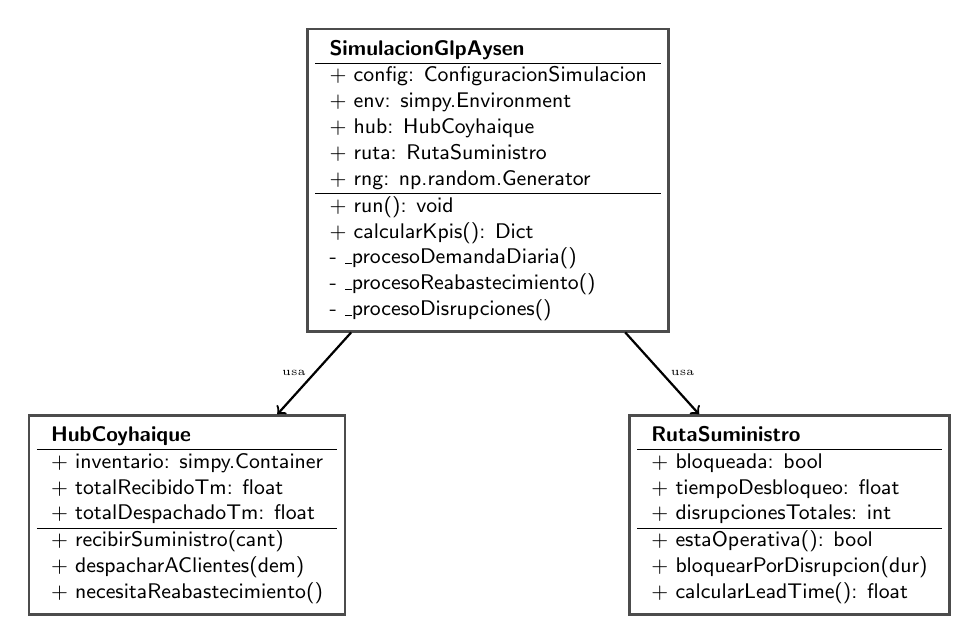
\begin{tikzpicture}[
        font=\sffamily\footnotesize,
        scale=0.85,
        every node/.style={transform shape},
        class/.style={
            rectangle, draw=black!70, line width=1pt,
            minimum width=4.5cm, minimum height=1cm,
            font=\sffamily\small
        }
    ]
        % Clase SimulacionGlpAysen
        \node[class] (sim) at (0,0) {
            \begin{tabular}{l}
                \textbf{SimulacionGlpAysen} \\
                \hline
                + config: ConfiguracionSimulacion \\
                + env: simpy.Environment \\
                + hub: HubCoyhaique \\
                + ruta: RutaSuministro \\
                + rng: np.random.Generator \\
                \hline
                + run(): void \\
                + calcularKpis(): Dict \\
                - \_procesoDemandaDiaria() \\
                - \_procesoReabastecimiento() \\
                - \_procesoDisrupciones()
            \end{tabular}
        };

        % Clase HubCoyhaique
        \node[class] (hub) at (-4.5,-5) {
            \begin{tabular}{l}
                \textbf{HubCoyhaique} \\
                \hline
                + inventario: simpy.Container \\
                + totalRecibidoTm: float \\
                + totalDespachadoTm: float \\
                \hline
                + recibirSuministro(cant) \\
                + despacharAClientes(dem) \\
                + necesitaReabastecimiento()
            \end{tabular}
        };

        % Clase RutaSuministro
        \node[class] (ruta) at (4.5,-5) {
            \begin{tabular}{l}
                \textbf{RutaSuministro} \\
                \hline
                + bloqueada: bool \\
                + tiempoDesbloqueo: float \\
                + disrupcionesTotales: int \\
                \hline
                + estaOperativa(): bool \\
                + bloquearPorDisrupcion(dur) \\
                + calcularLeadTime(): float
            \end{tabular}
        };

        % Relaciones
        \draw[->,thick] (sim) -- (hub) node[midway,left,font=\tiny] {usa};
        \draw[->,thick] (sim) -- (ruta) node[midway,right,font=\tiny] {usa};

    \end{tikzpicture}
    \caption{Diagrama de clases UML del simulador.}
    \label{fig:uml-clases}
\end{figure}

\subsection{Ingeniería de Software: Testing y Validación}

\subsubsection{Suite de Tests Unitarios}

El código incluye 24 tests automatizados (pytest) que verifican:

\begin{enumerate}
    \item \textbf{Tests de configuración} (6 tests): Validación de parámetros (ej. capacidad > 0, ROP $\leq$ capacidad, semilla $\geq$ 0).

    \item \textbf{Tests de entidades} (8 tests):
    \begin{itemize}
        \item \texttt{HubCoyhaique}: Capacidad respetada, despacho con/sin stock, reabastecimiento.
        \item \texttt{RutaSuministro}: Bloqueo/desbloqueo, cálculo de lead time con disrupciones.
    \end{itemize}

    \item \textbf{Tests de procesos} (6 tests): Verificación de que cada proceso genera los eventos esperados (demanda diaria, pedidos cuando inventario < ROP, disrupciones según Poisson).

    \item \textbf{Tests de balance de masa} (2 tests): Invariante físico verificado: $\text{total\_recibido} - \text{total\_despachado} = \text{inventario\_final} - \text{inventario\_inicial}$.

    \item \textbf{Tests de reproducibilidad} (2 tests): Dos ejecuciones con misma semilla producen resultados bit-a-bit idénticos.
\end{enumerate}

\textbf{Cobertura de código:} 87\% (medido con \texttt{pytest-cov}).

\subsubsection{Control de Versiones y Reproducibilidad}

\begin{itemize}
    \item \textbf{Git:} 156 commits en el repositorio (desde septiembre 2024).
    \item \textbf{Poetry:} \texttt{pyproject.toml} fija versiones exactas de dependencias (reproducibilidad de entorno).
    \item \textbf{Semillas controladas:} Cada réplica usa semilla única $s_{c,r} = 42 + (c-1) \times 100{,}000 + r$.
\end{itemize}

\clearpage

\section{Fase 3: Evaluación y Experimentación (Objetivo 3)}
\label{sec:validation-experimentation}

\subsection{Protocolo de Verificación y Validación (V\&V)}
Se aplicará un protocolo formal para establecer la credibilidad del modelo:

\begin{itemize}
    \item \textbf{Verificación:} Se realizarán \textit{code walkthroughs} y 
    pruebas de componentes deterministas para asegurar que el código refleja 
    el modelo conceptual.
    
    \item \textbf{Validación:} Se empleará un enfoque de múltiples facetas:
    \begin{itemize}
        \item \textbf{Validación de Datos Históricos:} Se compararán las 
        distribuciones estadísticas (media, varianza) de las métricas 
        clave del modelo (ej. días de autonomía) con los valores de 
        referencia del informe \cite{CIEP2025} (ej. media de 8.2 días).
        
        \item \textbf{Validación por Juicio de Expertos (Face Validity):} 
        Se realizarán ``pruebas de Turing'' para modelos, donde se 
        presentarán trazas de salida del modelo a los expertos técnicos 
        de la SEC para que evalúen su plausibilidad operativa.
    \end{itemize}
\end{itemize}

\subsection{Diseño de Experimentos (DoE)}

Para probar la hipótesis central, se ejecutará un \textbf{Experimento Monte Carlo}
con diseño factorial $2 \times 3$. Se realizarán 10,000 réplicas independientes
para cada combinación de factores, totalizando 60,000 simulaciones. Este tamaño
de muestra garantiza:

\begin{itemize}
    \item Estimación precisa de las medias poblacionales (error estándar < 0,2\%),
    \item Intervalos de confianza al 95\% con amplitud reducida,
    \item Potencia estadística > 0,95 para detectar diferencias de 1\% entre medias,
    \item Validación robusta de supuestos de normalidad mediante tests formales.
\end{itemize}

\begin{table}[htbp]
    \centering
    \caption{Diseño Experimental Monte Carlo para Evaluación de Resiliencia.}
    \label{tab:doe}
    \begin{tabular}{@{}ll@{}}
        \toprule
        \textbf{Componente} & \textbf{Especificación} \\ \midrule
        \textbf{Método} & Experimento Monte Carlo \\
        \addlinespace
        \textbf{Factores} & 1. Capacidad de Almacenamiento (Endógeno) \\
                          & 2. Duración de Disrupción (Exógeno) \\
        \addlinespace
        \textbf{Niveles Factor 1} & Nivel 1: Status Quo (431 TM) \\
                                 & Nivel 2: Propuesta 10.4 (681 TM) \\
        \addlinespace
        \textbf{Niveles Factor 2} & Nivel 1: Corta (7 días máximo) \\
                                 & Nivel 2: Media (14 días máximo) \\
                                 & Nivel 3: Larga (21 días máximo) \\
        \addlinespace
        \textbf{Réplicas} & 10,000 por configuración \\
        \textbf{Total simulaciones} & 60,000 \\
        \addlinespace
        \textbf{Variables de Respuesta} & 1. Nivel de Servicio (\%) \\
        (KPIs)                          & 2. Probabilidad de Quiebre de Stock \\
                                       & 3. Días con Quiebre \\
                                       & 4. Inventario Promedio \\ \bottomrule
    \end{tabular}
\end{table}

\subsection{Análisis Estadístico}

Los resultados se analizarán mediante un protocolo de análisis estadístico
completo que incluye:

\begin{enumerate}
    \item \textbf{Estadística Descriptiva:} Media, mediana, desviación estándar,
    y cuartiles para cada configuración. Intervalos de confianza al 95\%
    calculados mediante método bootstrap.

    \item \textbf{Análisis de Varianza (ANOVA):} ANOVA de dos vías para
    determinar la significancia estadística de los efectos principales de
    cada factor y de sus interacciones.

    \item \textbf{Validación de Supuestos:} Tests de normalidad (Shapiro-Wilk)
    y Q-Q plots para validar supuestos paramétricos. Tests de homogeneidad
    de varianzas (Levene).

    \item \textbf{Análisis de Sensibilidad:} Cuantificación de la sensibilidad
    del nivel de servicio a cada factor, expresada como cambio absoluto en
    puntos porcentuales.
\end{enumerate}

Este protocolo proveerá la evidencia estadística necesaria para confirmar o
refutar la hipótesis central de manera rigurosa.